\documentclass[lettersize,journal]{IEEEtran}
\usepackage{amsmath,amsfonts}
\usepackage{algorithmic}
\usepackage{array}
\usepackage[caption=false,font=normalsize,labelfont=sf,textfont=sf]{subfig}
\usepackage{textcomp}
\usepackage{stfloats}
\usepackage{url}
\usepackage{verbatim}
\usepackage{graphicx}
\hyphenation{op-tical net-works semi-conduc-tor IEEE-Xplore}
\def\BibTeX{{\rm B\kern-.05em{\sc i\kern-.025em b}\kern-.08em
    T\kern-.1667em\lower.7ex\hbox{E}\kern-.125emX}}
\usepackage{balance}

\hyphenpenalty=25
\tolerance=10000
\usepackage{tcolorbox}
\newcommand{\ciao}[1]{{\setlength\fboxrule{0pt}\fbox{\tcbox[colframe=black,colback=white,shrink tight,boxrule=0.5pt,extrude by=1mm]{\small #1}}}}
% \usepackage{fontspec}
% \usepackage{libertine}

\begin{document}
% \libertineGlyph{uni2460} \libertineGlyph{uni24F5} \libertineGlyph{uni2776}


\title{$H$-$D$ Support Set: Frequency Dynamic Security Analysis through Multidimensional Frequency Parameter Bindings}
\author{Yiping Yuan, Liqian Zhu,
\thanks{Manuscript created October, 2020; This work was developed by the IEEE Publication Technology Department. This work is distributed under the \LaTeX \ Project Public License (LPPL) ( http://www.latex-project.org/ ) version 1.3. A copy of the LPPL, version 1.3, is included in the base \LaTeX \ documentation of all distributions of \LaTeX \ released 2003/12/01 or later. The opinions expressed here are entirely that of the author. No warranty is expressed or implied. User assumes all risk.}}

\markboth{Journal of \LaTeX\ Class Files,~Vol.~18, No.~9, September~2020}%
{frequency dynamic identification through multi-dimensional frequency parameter bindings}

\maketitle

\begin{abstract}

  Existing research on the system frequency response (SFR) and frequency-constrained scheduling studies primarily relies on commonly-used metrics consisting of rate-of-frequency-change, nadir, and quasi-steady-state (QSS). Nevertheless, the complex interdependencies among these parameters have not been fully explored. This letter introduces a new criterion to assess frequency stability by directly considering multidimensional relationships between these frequency parameters. An analytical solution is derived to quantify these interdependencies, and a convex polygon representation is constructed to visualize the feasible operating region defined by these parameters. Using this criterion, the impact of different frequency parameter settings on system stability can be clearly obtained and analyzed. The effectiveness of the proposed approach is demonstrated on a modified IEEE 30-bus test system.

\end{abstract}

\begin{IEEEkeywords}
Class, IEEEtran, \LaTeX, paper, style, template, typesetting.
\end{IEEEkeywords}

\section{Introduction}
\IEEEPARstart{T}{he} low inertia character of electrical power system significantly impact the system frequency security, which implicitly change the scheduling commitment results provided by different generators. In such circumstances, existing studies about power system dynamic response, storage device sizing and control parameter tunning, optimal scheduling operation, and even medium-term~\&~long-term generation planning studies trends to emphasis the consideration of frequency response and frequency stability.


% The primary objective of frequency-oriented studies mentioned before is to determine the safety of frequency dynamic processes, as characterized by multidimensional frequency parameters such as inertia, damping and droop, reserves, etc. A conventional approach involves establishing dynamic frequency criteria, encompassing constraints on RoCoF, nadir, and QSS, typically expressed as mathematical relationships between these frequency parameters, to ensure frequency security. System stability is then assessed by evaluating whether the observed frequency dynamics remain within the feasible region defined by these criteria.  From this perspective, it is only possible to qualitatively assess whether the current configuration of frequency parameters is reasonable. However, it cannot refer the safety boundaries of multidimensional frequency parameters.

The primary objective of frequency-oriented studies as previously discussed is to ascertain the security of frequency dynamic, while it can be described through the SFR function, typically expressed by multidimensional frequency parameters, including system-level/regional-level $inertia$, $damping$, $droop$, and $reserve$, etc. Conventional methodologies establish dynamic frequency criteria, typically expressed as mathematical inequalities such as RoCoF, nadir and QSS. These criteria define a feasible operating region within which frequency dynamics are deemed secure. System stability is subsequently evaluated by determining if the observed frequency derivation derived from the SFR function remains within this defined region.

Nevertheless, these conventional approaches suffers from an implicitly limitation: it provides only a qualitative assessment of the current frequency parameter configuration's reasonableness. While it can determine if the system operates within predefined (frequency dynamic) limits, it fails to explicitly delineate the precise safety boundaries of these multidimensional frequency parameters. Consequently, it can neither directly quantify the margins of safety, nor provide actionable insights into how to adjust these parameters to enhance system frequency security.


This letter introduces the new concept of the $H$-$D$ Support Set, which characterizes the feasible boundary of multidimensional frequency parameters. Furthermore, an open-source tool (repo address: \url{https://github.com/Divas1234/frequencyregions.git}) for $H$-$D$ Support Set simulation is made freely available. Leveraging the SFR theorem, the interaction between these parameters is analyzed, and both the upper and lower bounds of the parameter space are explicitly calculated. In contrast to existing methodologies, the proposed approach provides a well-defined boundary interval for frequency parameters, thereby enabling more effective tuning optimization of frequency control parameters and facilitating comprehensive frequency dynamic analysis.

\section{SFR theorem in low inertia power systems}

Given such a low inertia power systems that considers high penetration of converters, the uniform analytical expression of frequency dynamic processes can be written as,

\begin{subequations}

% The primary objective of frequency-oriented studies mentioned before is to determine the safety of frequency dynamic processes, as characterized by multidimensional frequency parameters such as inertia, damping and droop, reserves, etc. A conventional approach involves establishing dynamic frequency criteria, encompassing constraints on RoCoF, nadir, and QSS, typically expressed as mathematical relationships between these frequency parameters, to ensure frequency security. System stability is then assessed by evaluating whether the observed frequency dynamics remain within the feasible region defined by these criteria.  From this perspective, it is only possible to qualitatively assess whether the current configuration of frequency parameters is reasonable. However, it cannot refer the safety boundaries of multidimensional frequency parameters.

The primary objective of frequency-oriented studies as previously discussed is to ascertain the security of frequency dynamic, while it can be described through the SFR function, typically expressed by multidimensional frequency parameters, including system-level/regional-level $inertia$, $damping$, $droop$, and $reserve$, etc. Conventional methodologies establish dynamic frequency criteria, typically expressed as mathematical inequalities such as RoCoF, nadir and QSS. These criteria define a feasible operating region within which frequency dynamics are deemed secure. System stability is subsequently evaluated by determining if the observed frequency derivation derived from the SFR function remains within this defined region.

Nevertheless, these conventional approaches suffers from an implicitly limitation: it provides only a qualitative assessment of the current frequency parameter configuration's reasonableness. While it can determine if the system operates within predefined (frequency dynamic) limits, it fails to explicitly delineate the precise safety boundaries of these multidimensional frequency parameters. Consequently, it can neither directly quantify the margins of safety, nor provide actionable insights into how to adjust these parameters to enhance system frequency security.


This letter introduces the new concept of the $H$-$D$ Support Set, which characterizes the feasible boundary of multidimensional frequency parameters. Furthermore, an open-source tool (repo address: \url{https://github.com/Divas1234/frequencyregions.git}) for $H$-$D$ Support Set simulation is made freely available. Leveraging the SFR theorem, the interaction between these parameters is analyzed, and both the upper and lower bounds of the parameter space are explicitly calculated. In contrast to existing methodologies, the proposed approach provides a well-defined boundary interval for frequency parameters, thereby enabling more effective tuning optimization of frequency control parameters and facilitating comprehensive frequency dynamic analysis.

\section{SFR theorem in low inertia power systems}

Given such a low inertia power systems that considers high penetration of converters, the uniform analytical expression of frequency dynamic processes can be written as,

\begin{subequations}
\begin{align}
  \!\!\!\!&\varDelta f(s) \!=\! \frac{1+sT}{2H_{EQU}T_{G}(s^2 + 2\zeta \omega_n s + \omega_n^2)}\frac{\varDelta P_{Step}}{s}\label{eq:Lsfr}\\
  \!\!\!\!&\omega_n \!=\! \sqrt{\!\frac{D_{EQU} \!+\! R_G}{2H_{EQU}T_G}}, \zeta \!=\! \frac{2H_{EQU}  \!+\! T_G(D_{EQU} \!+\! F_G)}{2\sqrt{2H_{EQU}T_G(D_{EQU} \!+\! R_G)}}
  \!\!\!\!&\varDelta f(s) \!=\! \frac{1+sT}{2H_{EQU}T_{G}(s^2 + 2\zeta \omega_n s + \omega_n^2)}\frac{\varDelta P_{Step}}{s}\label{eq:Lsfr}\\
  \!\!\!\!&\omega_n \!=\! \sqrt{\!\frac{D_{EQU} \!+\! R_G}{2H_{EQU}T_G}}, \zeta \!=\! \frac{2H_{EQU}  \!+\! T_G(D_{EQU} \!+\! F_G)}{2\sqrt{2H_{EQU}T_G(D_{EQU} \!+\! R_G)}}
\end{align}
\end{subequations}

\noindent
where $\varDelta f(s)$ represents the frequency derivation with a step-type power disturbance $\varDelta P_{Step}$, $H_{EQU},\! D_{DEQ}$, respectively, describes the equivalent inertia parameter and damping parameter, $T_G$ is the time constant of conventional generator, $R_G$ denotes the aggregated droop parameter generated by conventional generators, $F_G$ denote the fraction of total power generated by high pressure turbines of conventional generators. In these formulations, the time constants within the transfer function of $\varDelta f(s)$ are normalized to unity, and the response times of converters with diverse control schemes are approximated as negligible. A more detailed feasibility analysis is provided in [].

In correlation with (1), the maximum frequency deviation termed as $\max[ \varDelta f(t)]$ as well as the maximization rate of frequency change termed as $\max[\varDelta f'(t)]$ can be derived as below,

\begin{subequations}
\end{subequations}

\noindent
where $\varDelta f(s)$ represents the frequency derivation with a step-type power disturbance $\varDelta P_{Step}$, $H_{EQU},\! D_{DEQ}$, respectively, describes the equivalent inertia parameter and damping parameter, $T_G$ is the time constant of conventional generator, $R_G$ denotes the aggregated droop parameter generated by conventional generators, $F_G$ denote the fraction of total power generated by high pressure turbines of conventional generators. In these formulations, the time constants within the transfer function of $\varDelta f(s)$ are normalized to unity, and the response times of converters with diverse control schemes are approximated as negligible. A more detailed feasibility analysis is provided in [].

In correlation with (1), the maximum frequency deviation termed as $\max[ \varDelta f(t)]$ as well as the maximization rate of frequency change termed as $\max[\varDelta f'(t)]$ can be derived as below,

\begin{subequations}
\begin{align}
    \max[\Delta f(t)] &= \varDelta f(t)|_{t=t_{nadir}^k} = -\frac{\Delta P_{Step}}{D_{EQU} + R_G} \left( 1 + \right.\notag \\
                      &\left. (-1)^k \sqrt{\frac{T_G(R_G - F_G)}{2H_{EQU}}} e^{-\zeta \omega_n t_{nadir}^k} \right) \label{eq:max_delta_f}\\
    t_{nadir}^k &= \frac{1}{\omega_d} \arctan \left( \frac{\omega_d}{\zeta \omega_n - T_G^{-1}} \right) + \frac{k\pi}{\omega_d}\notag  \\
    \omega_d &= \omega_n \sqrt{1 - \zeta^2}, \quad \phi = \sin^{-1} \left( \sqrt{1 - \zeta^2} \right) \notag\\
  \max[\varDelta f'(t)] &= \varDelta f'(t)|_{t=t_{0}} = \frac{1}{2} H_{EQU}^{-1}\varDelta P_{Step} \label{eq:max_rocof}\\
  \varDelta f_{QSS}(t) &= \varDelta f(t)|_{t=t_{\infty}} = {D_{EQU}^{-1}\varDelta P_{Step}} \label{eq:qss}
    \max[\Delta f(t)] &= \varDelta f(t)|_{t=t_{nadir}^k} = -\frac{\Delta P_{Step}}{D_{EQU} + R_G} \left( 1 + \right.\notag \\
                      &\left. (-1)^k \sqrt{\frac{T_G(R_G - F_G)}{2H_{EQU}}} e^{-\zeta \omega_n t_{nadir}^k} \right) \label{eq:max_delta_f}\\
    t_{nadir}^k &= \frac{1}{\omega_d} \arctan \left( \frac{\omega_d}{\zeta \omega_n - T_G^{-1}} \right) + \frac{k\pi}{\omega_d}\notag  \\
    \omega_d &= \omega_n \sqrt{1 - \zeta^2}, \quad \phi = \sin^{-1} \left( \sqrt{1 - \zeta^2} \right) \notag\\
  \max[\varDelta f'(t)] &= \varDelta f'(t)|_{t=t_{0}} = \frac{1}{2} H_{EQU}^{-1}\varDelta P_{Step} \label{eq:max_rocof}\\
  \varDelta f_{QSS}(t) &= \varDelta f(t)|_{t=t_{\infty}} = {D_{EQU}^{-1}\varDelta P_{Step}} \label{eq:qss}
\end{align}
\end{subequations}
  
\noindent
where $\max [\varDelta f(t)]^k$ enforces the maximum frequency deviation at the $k$-th cycle, $\max [\varDelta f'(t)]$ defines the maximum rate of change of frequency derivation, $\varDelta f_{QSS} (t)$ denotes the (quasi) steady-state frequency deviation, $t_{nadir}^k$ denotes the time to the $k$-th nadir of the frequency deviation.

\begin{figure}
  \centering
  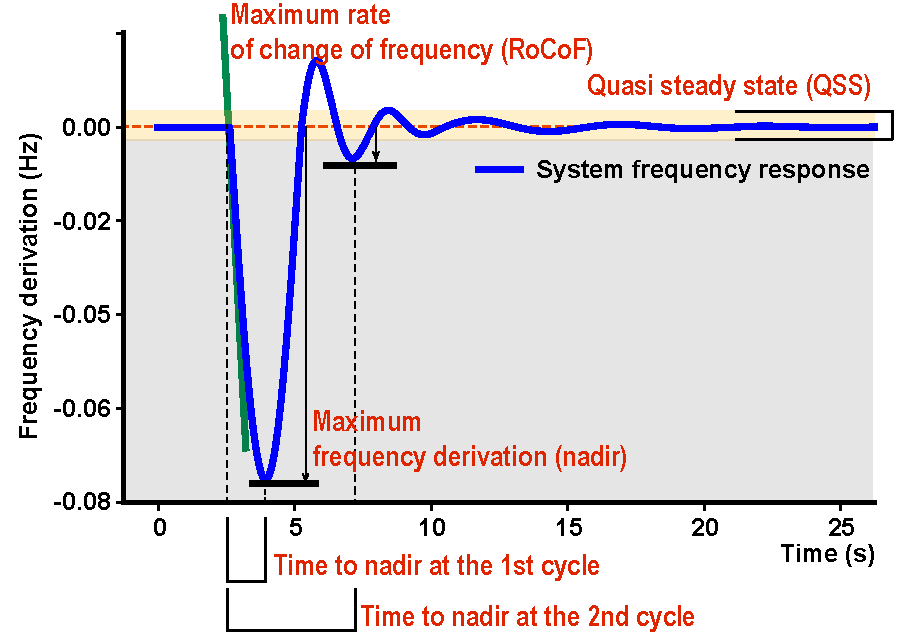
\includegraphics[width=0.48\textwidth]{frequency_response.pdf}
  \caption{system frequency response}
  \label{fig:myimage}
\end{figure}

To ensure the security of frequency dynamics across the entire frequency response processes, the amounts of $\max[\varDelta f(t)]$, $\max[\varDelta f'(t)]$ and $\varDelta f_{QSS}(t)$ must be constrained within the predefined frequency dynamic restrictions, as discussed in existing frequency-oriented studies,

\begin{subequations}
  \begin{align}
  \left \{
  \begin{array}{rr}
  {Nadir\,\, constraint:}& \max[\varDelta f (t)] \leq \gamma_{Nadir}\\
  {RoCoF\,\, constraint:}&\max[\varDelta f' (t)] \leq \gamma_{RoCoF}\\
  {QSS\,\, constraint:} &\varDelta f_{QSS} (t) \leq \gamma_{QSS}\\
\end{array}
\right.
    \end{align}
  \end{subequations}

  \noindent
where $\gamma_{Nadir}$, $\gamma_{RoCoF}$ and $\gamma_{QSS}$ are predefined frequency dynamic restrictions concerning frequency nadir, RoCoF, and QSS frequency derivation, respectively.

\section{$H$-$D$ support set: A new criterion for frequency security identification}  

This section derives explicit bounds of multidimensional frequency parameters, including inertia, damping, and droop gains, these bindings result in a new criterion for frequency security identification that differs from (3a).

The sufficient condition for the occurrence of maximum frequency derivation (nadir) is predicated on the convergence of the transfer function (1a) and the non-negativity characteristic of time-to-nadir coefficient. For the first category, this translates to the mathematical requirement that all poles, as derived from the denominator of (1a), must lie within the left half of the complex $s$-plane. Since the amount of poles in (1a) can be written as $-\zeta \omega_n \pm \omega_n \sqrt{1 - \zeta^2}$, $\zeta \geq 0$ must hold to ensure the convergence of the transfer function. For the latter category, the amount of denominator should be positive to guarantee the non-negativity of time-to-nadir coefficient, that is, $\zeta \omega_n - T_G^{-1}\geq 0, \text{and}\, \sqrt{1-\zeta^2} \geq 0$. So, the determination conditions for the intermediate variables, $\zeta, \omega_n$, can be obtained,

\begin{subequations}
  \begin{align}
    0 \leq \zeta \leq 1, \quad \zeta \omega_n \geq \frac{1}{T_G} \label{eq:zeta_wn}
    \end{align}
  \end{subequations}

Substituting (1b) into (4a), the bounds of inertia and damping parameters can be derived as below,

\begin{subequations}
  \begin{align}
    H_{EQU} &\leq \frac{1}{2}T_G \left(\text{term}_1 + \sqrt{\text{term}_2} \right) \\
    H_{EQU} &\geq \frac{1}{2}T_G \left(\text{term}_1 - \sqrt{\text{term}_2} \right) \\
    \text{term}_1 &= (D_{EQU} - F_G + 2R_G) \\
    \text{term}_2 &= {(D_{EQU} - F_G + 2R_G)^2 - (D_{EQU} + F_G)^2}\\
    \text{term}_2 &\geq 0 \Longrightarrow (R_G - F_G)(R_G + D_{EQU}) \geq 0
    \end{align}
  \end{subequations}

Let $H_{EQU}=\mathcal{Q} (D_{EQU})$, the relationship between $H_{EQU}$ and $D_{EQU}$ can be derived as below,

\begin{subequations}
  \begin{align}
    \overbrace{\frac{1}{2}T_G \left(\text{term}_1 - \sqrt{\text{term}_2} \right)}^{lower\,bound} \leq H_{EQU}=\mathcal{Q} (D_{EQU}) \leq \notag \\
    \underbrace{\frac{1}{2}T_G \left(\text{term}_1 + \sqrt{\text{term}_2} \right)}_{upper\, bound}, (R_G - F_G) \geq 0
    \end{align}
  \end{subequations}

Next, other relations between $H_{EQU}$ and $D_{EQU}$ concerning nadir, RoCoF, and Qss, can be extended from (3a). For simplification, let $\max [ \varDelta f(t)]=\mathcal{R} (H_{EQU}, D_{EQU})$ denotes the non-linear close form of (2a), then, more bindings between $H_{EQU}$ and $D_{EQU}$ can be derived as below,

\begin{subequations}
  \begin{align}
\overbrace{\frac{1}{2} \gamma_{RoCoF}^{-1} \varDelta P_{Step}}^{lower\, bound} \leq H_{EQU} &\leq \underbrace{\mathcal{R}^{-1}(D_{EQU}) \gamma_{Nadir}}_{upper\, bound} \\
D_{EQU} & \geq \gamma_{QSS}^{-1} \varDelta P_{Step}
  \end{align}
\end{subequations}

% \textcircled{\small{2}}
By further meticulously organizing the preceding derivations, a concise bounds for system inertia and damping parameters can be estimated from (6) and (7).

\begin{subequations}
  \begin{align}
    \!\!\!\begin{array}{rl}
    Inertia\,\, \ciao{1}\, lower\,bound:&\!\!\!\frac{1}{2} \gamma_{RoCoF}^{-1} \varDelta P_{Step}\\
    \ciao{2}\,lower\,bound:&\!\!\!\frac{1}{2}T_G \left(\text{term}_1 - \sqrt{\text{term}_2} \right)\\
    \ciao{3}\,upper\,bound:&\!\!\!\mathcal{R}^{-1}(D_{EQU}) \gamma_{Nadir} \\
    \ciao{4}\,upper\,bound:&\!\!\!\frac{1}{2}T_G \left(\text{term}_1 + \sqrt{\text{term}_2} \right)\\    
    Damping \,\,\ciao{5}\,lower\,bound:&\!\!\! \gamma_{QSS}^{-1} \varDelta P_{Step}\\ 
    \end{array}
  \end{align}
\end{subequations}


\end{document}


